\appendix
\pagenumbering{Alph}
\renewcommand{\thechapter}{\Alph{chapter}}
\renewcommand{\thesection}{\Roman{section}}
\renewcommand{\thesubsection}{\Roman{subsection}}
\renewcommand\floatpagefraction{0.1}
\clearpage
\chapter{Anhang}
\label{appendix:annex}

\section{Bilder}
\label{annex:images}

\begin{figure}[ht!]
  \begin{centering}
    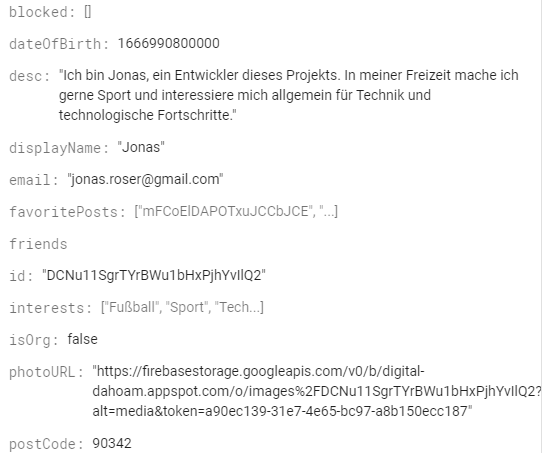
\includegraphics[width=1\textwidth]{figures/implementation/firestore-user.png}
    \caption{Benutzerdatensatz in Firestore}
    \label{fig:firestoreUser}
  \end{centering}
\end{figure}

\begin{figure}[ht!]
  \begin{centering}
    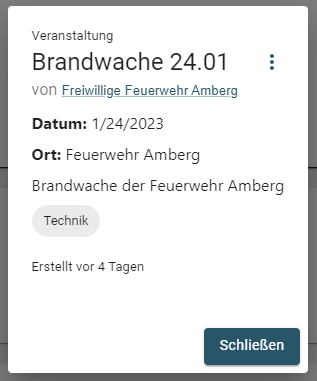
\includegraphics[width=.75\textwidth]{figures/implementation/details.png}
    \caption{Beitragsdetails}
    \label{fig:details}
  \end{centering}
\end{figure}

\clearpage
\section{Code}
\label{annex:code}

\begin{lstlisting}[language=JavaScript, label=code:filterPosts, title={Filterfunktion der Beiträge}]
const filtered = posts
.filter((post) => !currentUser?.blocked?.includes(post.author.id))
.filter((post) => {
  // check validity
  if (currentUser?.id === post.author.id) {
    return true
  }

  if (!(post.validityStart && post.validityEnd)) {
    // no validity set
    return true
  }
  console.log(
    moment(post.validityStart).toDate().getTime(),
    moment(post.validityStart).toDate().getTime() <= new Date().getTime(),
  )
  if (
    moment(post.validityStart).toDate().getTime() >= new Date().getTime() &&
    moment(post.validityEnd).toDate().getTime() <= new Date().getTime()
  ) {
    return true
  } else {
    return false
  }
})
\end{lstlisting}
